\chapter{基于图神经网络的流场模拟加速方法}

本章介绍了基于图神经网络的气动流场模拟加速方法,
首先利用CFD网格生成软件在算例几何模型上生成非结构网格,
基于网格单元拓扑连接信息、边界条件和初始条件提取图神经网络训练的输入数据;
利用CFD求解器获取图神经网络训练的真值。
然后基于图卷积神经网络设计了气动流场模拟加速模型,在模型训练完成后,
使用CFD求解器对气动流场模拟加速模型的输出结果进行优化。
最后在测试集上比较了气动流场模拟加速方法与传统CFD数值模拟方法的气动流场模拟效率。

\section{引言}

\subsection{动机分析}

利用深度学习方法对气动流场进行预测的主要思想是将气动流场模拟问题转化为图像回归预测问题,
因此需要将流场数据转化为矩阵的形式。
在处理流场中非结构数据时,则需要通过采样的方式将数据转化为结构规则的笛卡尔网格形式,
这样就会导致预测的结果在平滑区域(远场)过采样,而在流场边界层(几何体附近区域)欠采样,
导致预测流场结果在几何体周围轮廓模糊,不能真实的反映物理量在边界层的分布。
在传统基于网格的CFD模拟方法中,
一般通过加密边界层的网格密度以更加细致地捕捉边界层的速度和压力等物理量的变化,
使用均一的粗粒度的网格进行模拟根本不能得到准确的结果甚至导致计算不收敛。
此外,流场预测结果由深度学习模型输出,在复杂流动条件下,无法保证深度学习模型能够对流体运动规律进行准确学习,输出符合流体运动规律的预测结果。

基于以上考虑,本文在利用图神经网络进行流场模拟方面进行了探索,对气动流场模拟的效率和预测结果的有效性进行了权衡,
提出了基于图神经网络的流场模拟加速方法。

\subsection{研究思路}
与基于传统卷积神经网络的流场预测方法相比,基于图神经网络的流场模拟加速方法主要有两点不同:
1)流场数据表示方法通用性更强。
无论是结构网格还是非结构网格,利用图能够灵活地对网格单元的拓扑结构进行表示,
边界条件和初始条件可以处理为节点特征向量。
由于图结构利用网格对流场域进行了全尺寸模拟,不需要利用采样方法将流场表示为笛卡尔网格,
所以最大程度保留了原始流场数据中的信息,一些控制流体流动的全局变量也可以在图神经网络训练时用于每一个图节点上。
2)从根本上保证流场模拟结果的有效性。
利用CFD求解器对深度学习模型的预测结果进行优化,将计算收敛的结果作为最终的流场预测结果。
虽然深度学习模型在此方法中只是作为加速模块部分代替了CFD求解器的工作,
导致气动流场模拟效率低于基于深度学习的流场预测方法,
但由于气动流场模拟结果最终由CFD求解器输出,因此预测结果满足计算收敛条件和流体流动物理规律。




\subsection{OpenFOAM网格数据结构和图结构数据表示}\label{meshstructure}
本文基于OpenFOAM求解器进行网格生成和流场模拟,
OpenFOAM不支持二维网格,对于导入的外部二维网格,OpenFOAM会自动给网格加一个厚度,然后将前后面边界条件设置为空。
OpenFOAM主要网格文件及其包含的信息如表\ref{tab:openfoammesh}所示。

\begin{table}[htp]
	\setlength{\belowcaptionskip}{0.0cm}
	\caption{OpenFOAM网格文件信息}
	\label{tab:openfoammesh}
	\centering
	\begin{tabular}{c|c}
		\toprule
		文件 & 存储信息\\
		\midrule
		points  & 所有节点的三维坐标\\
		\midrule
		faces & 构造面单元的节点编号\\
		\midrule
		owner & 与面单元相对应owner体单元编号\\
		\midrule
		neighbour & 与面单元相对应neighbour体单元编号\\
		\midrule
		boundary & 边界条件设置\\		
		\bottomrule
	\end{tabular}
\end{table}

\texttt{points}文件以矢量场的形式存储所有节点坐标,单位为米,
文件主要内容如图\ref{fig:points_file}所示,节点的编号即为其坐标数据在points列表中的位置,初始编号为0。

\begin{figure}[htp]
	\centering
	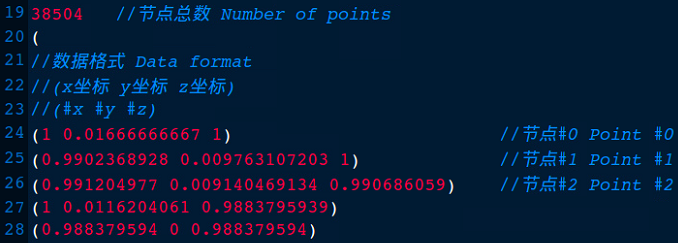
\includegraphics[width=0.72\textwidth]{./figures/points.png}
	\caption{points文件结构}
	\label{fig:points_file}	
\end{figure}

\texttt{faces}文件存储面单元-节点拓扑结构数据,文件主要内容如图\ref{fig:faces_file}所示。面单元最少由3个节点组成(三角形),其构造节点总数为每一行数据第一个整数(任意不小于3的值),每一行括号内的整数为面单元构造节点的编号,表示其在points列表中的位置。
面单元的编号即为数据在faces列表中的位置,初始编号为0。整个faces列表包含边界面单元。

\begin{figure}[htp]
	\centering
	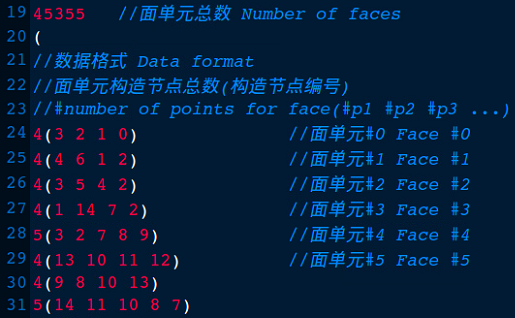
\includegraphics[width=0.72\textwidth]{./figures/faces.png}
	\caption{faces文件结构}
	\label{fig:faces_file}	
\end{figure}

如图\ref{fig:owner_neighbor}所示,owner体单元与neighbour体单元的标识基于公共面单元face外法向量($S_f$)的方向,即由owner单元指向neighbour单元。owner单元与neighbour单元有时亦被称为左单元与右单元。


\begin{figure}[htb]
	\centering
	\subfloat[]{\label{fig:on_2d}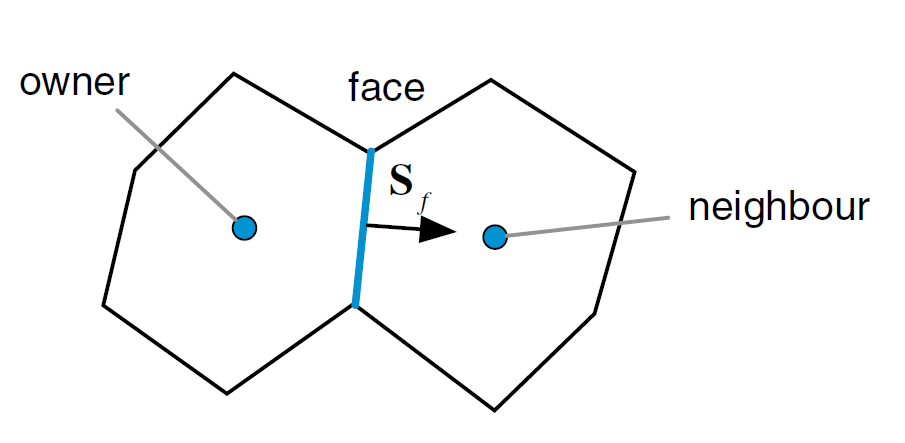
\includegraphics[width=0.45\textwidth]{figures/owner_neighbour_2d.png}} \qquad
	\subfloat[]{\label{fig:on_3d}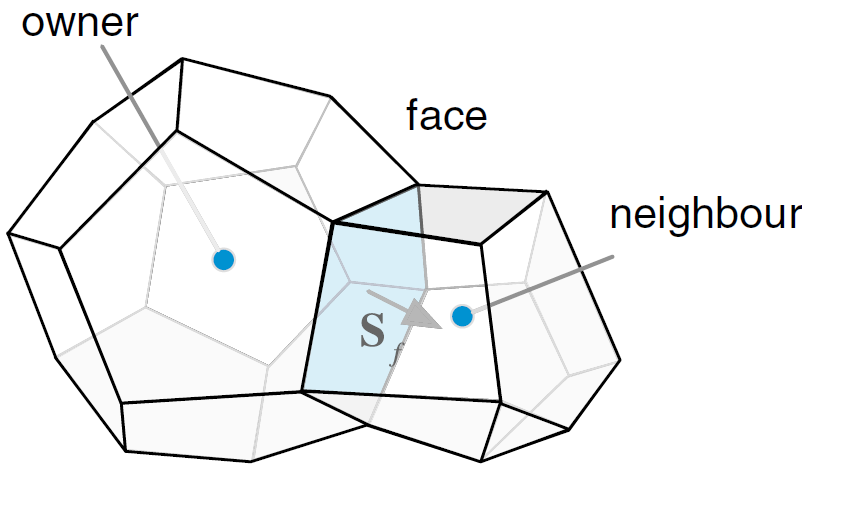
\includegraphics[width=0.45\textwidth]{figures/owner_neighbour.png}} 
	\caption{面的owner与neighbor的关系}
	\label{fig:owner_neighbor}
\end{figure}

\texttt{owner}文件存储owner单元-面单元拓扑结构数据,文件主要内容如图\ref{fig:owner_file}所示。owner列表存储相对应面单元的owner单元编号,初始编号为0,owner列表的位置对应面单元的编号,亦对应于其在faces列表中的位置。任何一个面单元总存在一个owner单元,因此owner单元总数与面单元总数nFaces相等。

\begin{figure}[htp]
	\centering
	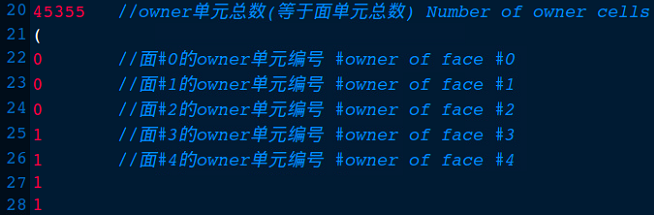
\includegraphics[width=0.72\textwidth]{./figures/owner.png}
	\caption{owner文件结构}
	\label{fig:owner_file}	
\end{figure}

\texttt{neighbour}文件存储neighbour单元-面单元拓扑结构数据,文件主要内容如图\ref{fig:neighbour_file}所示。neighbour列表存储相对应面单元的neighbour单元编号,初始编号不为0,neighbour列表的位置对应面单元的编号,亦对应于其在faces列表中的位置。需要特别说明的是,因为边界面单元没有neighbour单元,neighbour单元总数与内部面单元总数nInternalFaces相等。

\begin{figure}[htp]
	\centering
	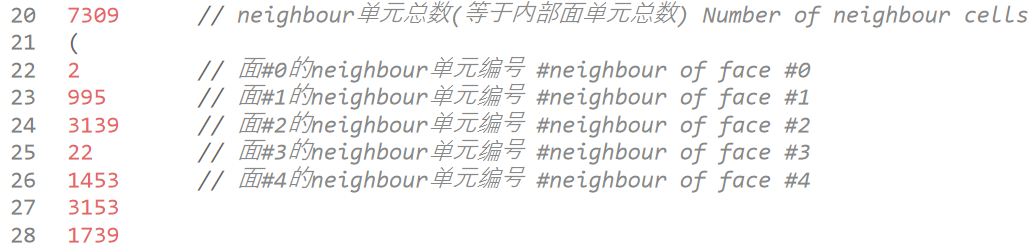
\includegraphics[width=0.72\textwidth]{./figures/neighbour.png}
	\caption{neighbour文件结构}
	\label{fig:neighbour_file}	
\end{figure}

\texttt{boundary}文件存储整个网格的边界信息,比如边界区域名称、边界类型type、面单元个数nFaces以及起始面单元编号startFace等,文件主要内容如图\ref{fig:boundary_file}所示。

\begin{figure}[htp]
	\centering
	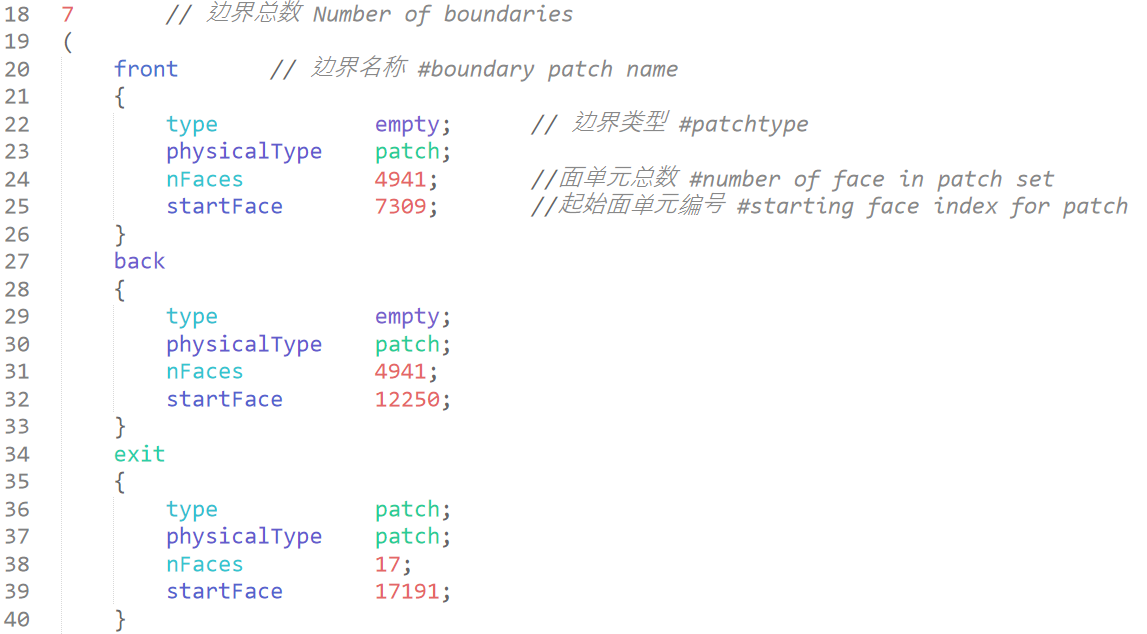
\includegraphics[width=0.72\textwidth]{./figures/boundary.png}
	\caption{boundary文件结构}
	\label{fig:boundary_file}	
\end{figure}


本文定义图结构$G=\left(X, E_{G}\right)$来表示OpenFOAM网格信息,
其中$X \in R^{N \times d}$表示图节点,节点数目为N,节点特征维度为d。
$E_{G}$表示边,每条边连接两个图节点,考虑到流体在网格中是相互流通的,所有的边均定义为无向边。

不同于基于网格节点进行流场模拟的求解器SU2\cite{2015SU2},OpenFOAM是基于有限体积方法离散的求解器,
基于控制体单元进行流场计算和模拟。因此,每个节点对应网格中的体单元,节点数和体单元总数相同;
对于二维流场,节点特征值包括体心坐标($C_x$,$C_y$),体单元的边界属性。
其中体心坐标可以通过\texttt{points}文件中点坐标进行插值得到;
体单元的边界属性由\texttt{boundary}文件中所属面单元的边界类型决定。
此外,本文将更多流场信息嵌入图节点特征向量中,包括控制流体流动的马赫数、攻角等全局变量,
利用距离符号函数计算的给定图节点到几何边界的最短距离。
每条边对应两个体单元的共有面,边总数和内部面单元总数相同,两个体单元分别为该面单元的owner和neighbor。



\section{基于GCN网络的气动流场加速}
正文内容



\section{实验设置与结果分析}

\subsection{数据集与参数设置}

\subsubsection{基于OpenFOAM求解器生成数据集}
实验算例设置二维非定常可压湍流固体外部流场,几何外形选取为空气动力学中经常研究的翼型。
机翼一般都有对称面。平行于机翼的对称面截得的机翼截面,称为翼剖面,通常也称为翼型。
翼型的几何形状是机翼的基本几何特性之一。
翼型的气动特性,直接影响到机翼及整个飞行器的气动特性,在空气动力学理论和飞行器设计中具有重要的地位。
图\ref{fig:airfoil_example}展示了翼型e342和翼型NACA 0012的几何外形示意图\cite{UIUCsite}。
\begin{figure}[htb]
	\centering
	\subfloat[e432]{\label{fig:e432}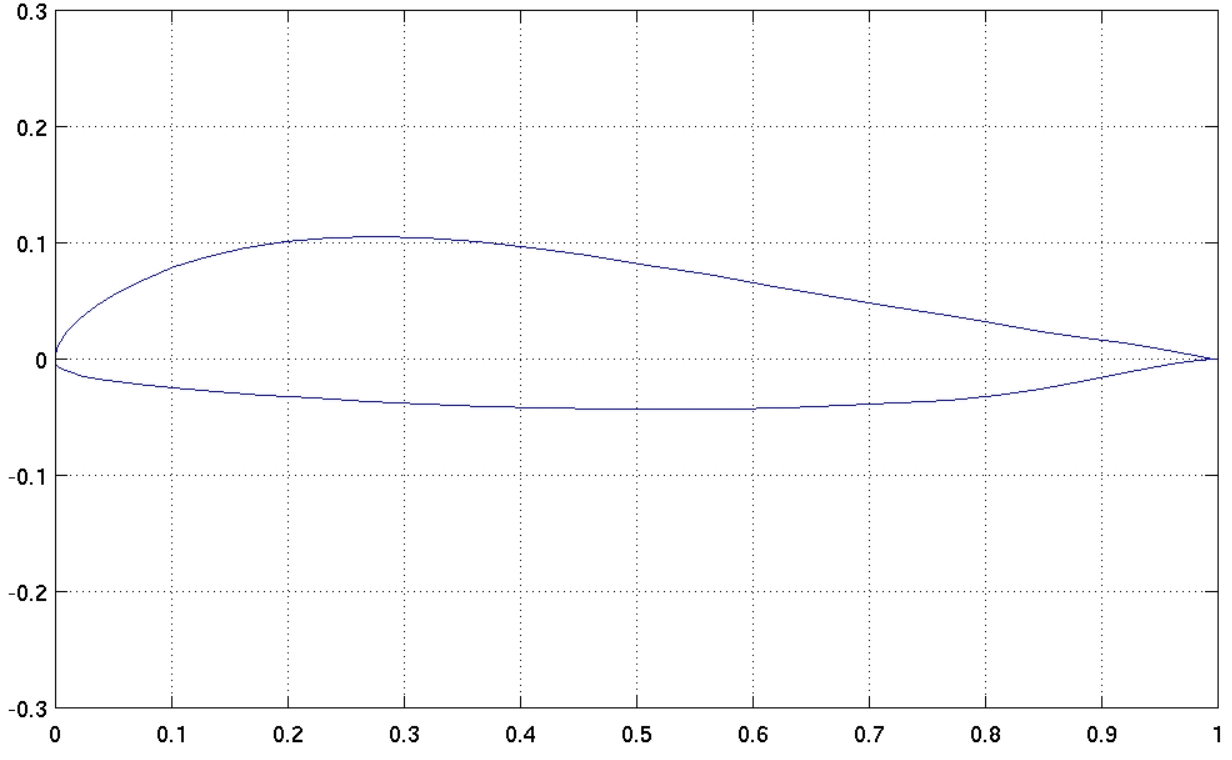
\includegraphics[width=0.42\textwidth]{figures/e342.png}} \qquad
	\subfloat[NACA 0012]{\label{fig:n0012}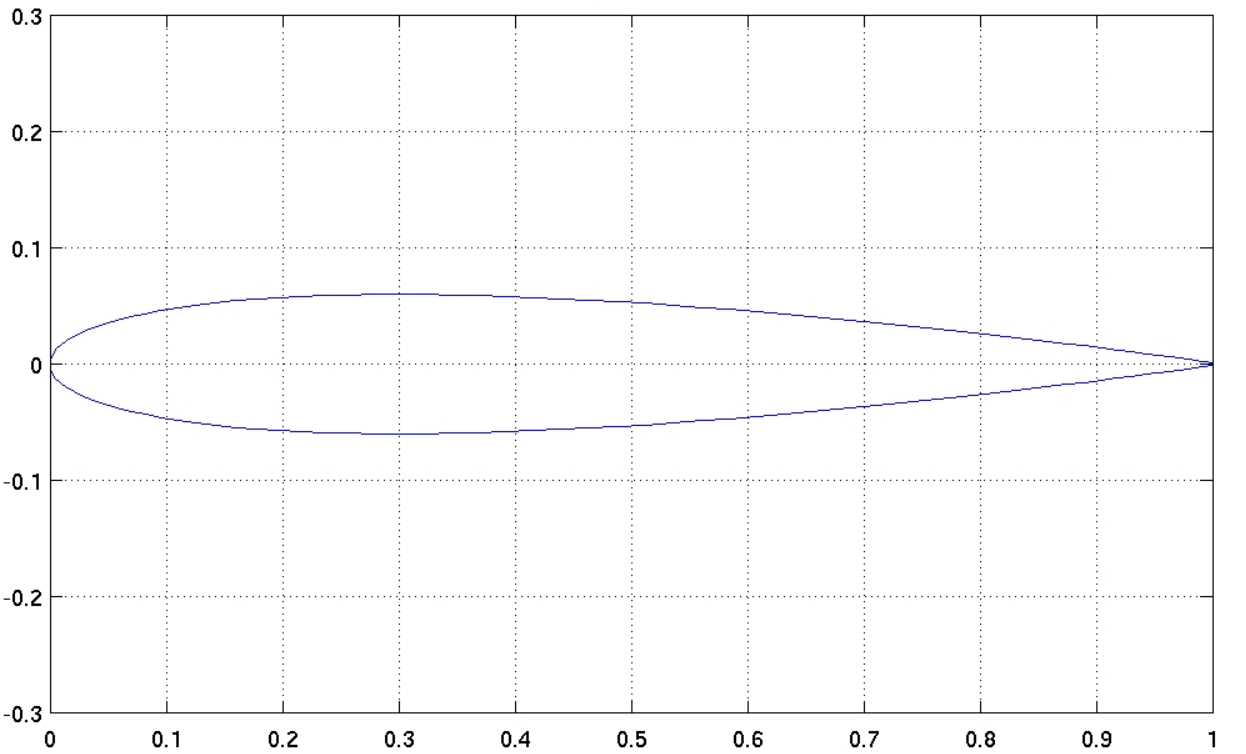
\includegraphics[width=0.42\textwidth]{figures/n0012.png}} 
	\caption{翼型e342和翼型NACA 0012几何外形示意图}
	\label{fig:airfoil_example}
\end{figure}

在获取翼型的几何模型之后,利用Gmsh\cite{gmsh}进行非结构网络的生成。
Gmsh是一个开源的具有内置CAD(Computer Aided Design)引擎和后期处理工具的三维有限元网格生成器,
可以方便地在Python脚本中调用Gmsh提供的接口对翼型进行网格生成。
全部网格信息保存在\texttt{.msh}文件中,再利用\texttt{gmshToFoam}指令将\texttt{.msh}文件导入OpenFOAM中,
就能得到\ref{meshstructure}节介绍的网格文件,完成网格生成任务。

\subsection{实验结果与分析}

层数、隐藏节点数、其他的超参数

\section{本章小结}

